\chapter{Evaluation}
To ensure that the prototype satisfied our final problem statement, we had to evaluate our prototype through an usability and user experience combined test. 

\section{The usability test}
In order to find out to which degree our prototype met our usability and user experience requirements, we conducted a combined usability and user experience test

\subsection{Test goals}
The main goal of this test was to figure out if our target group perceived the prototype's usability and that the user experience was satisfaction. Although our original idea was that this test should be tested on our experts, unfortunately this was not possible which led us to test the prototype on regular students from AAU CPH, but in role as a garden designer and the customer.\\
Efficiency??\\
Learnability??\\
Safety???\\

\subsection{Sampling}
The combined usability test was conducted with the help of (number) participants. We used convenience sampling to find students at AAU CPH.

\subsection{Test specifics}
In \autoref{fig:test1} seen below, is the setup for our usability test.

\begin{figure}[H]
	\centering
	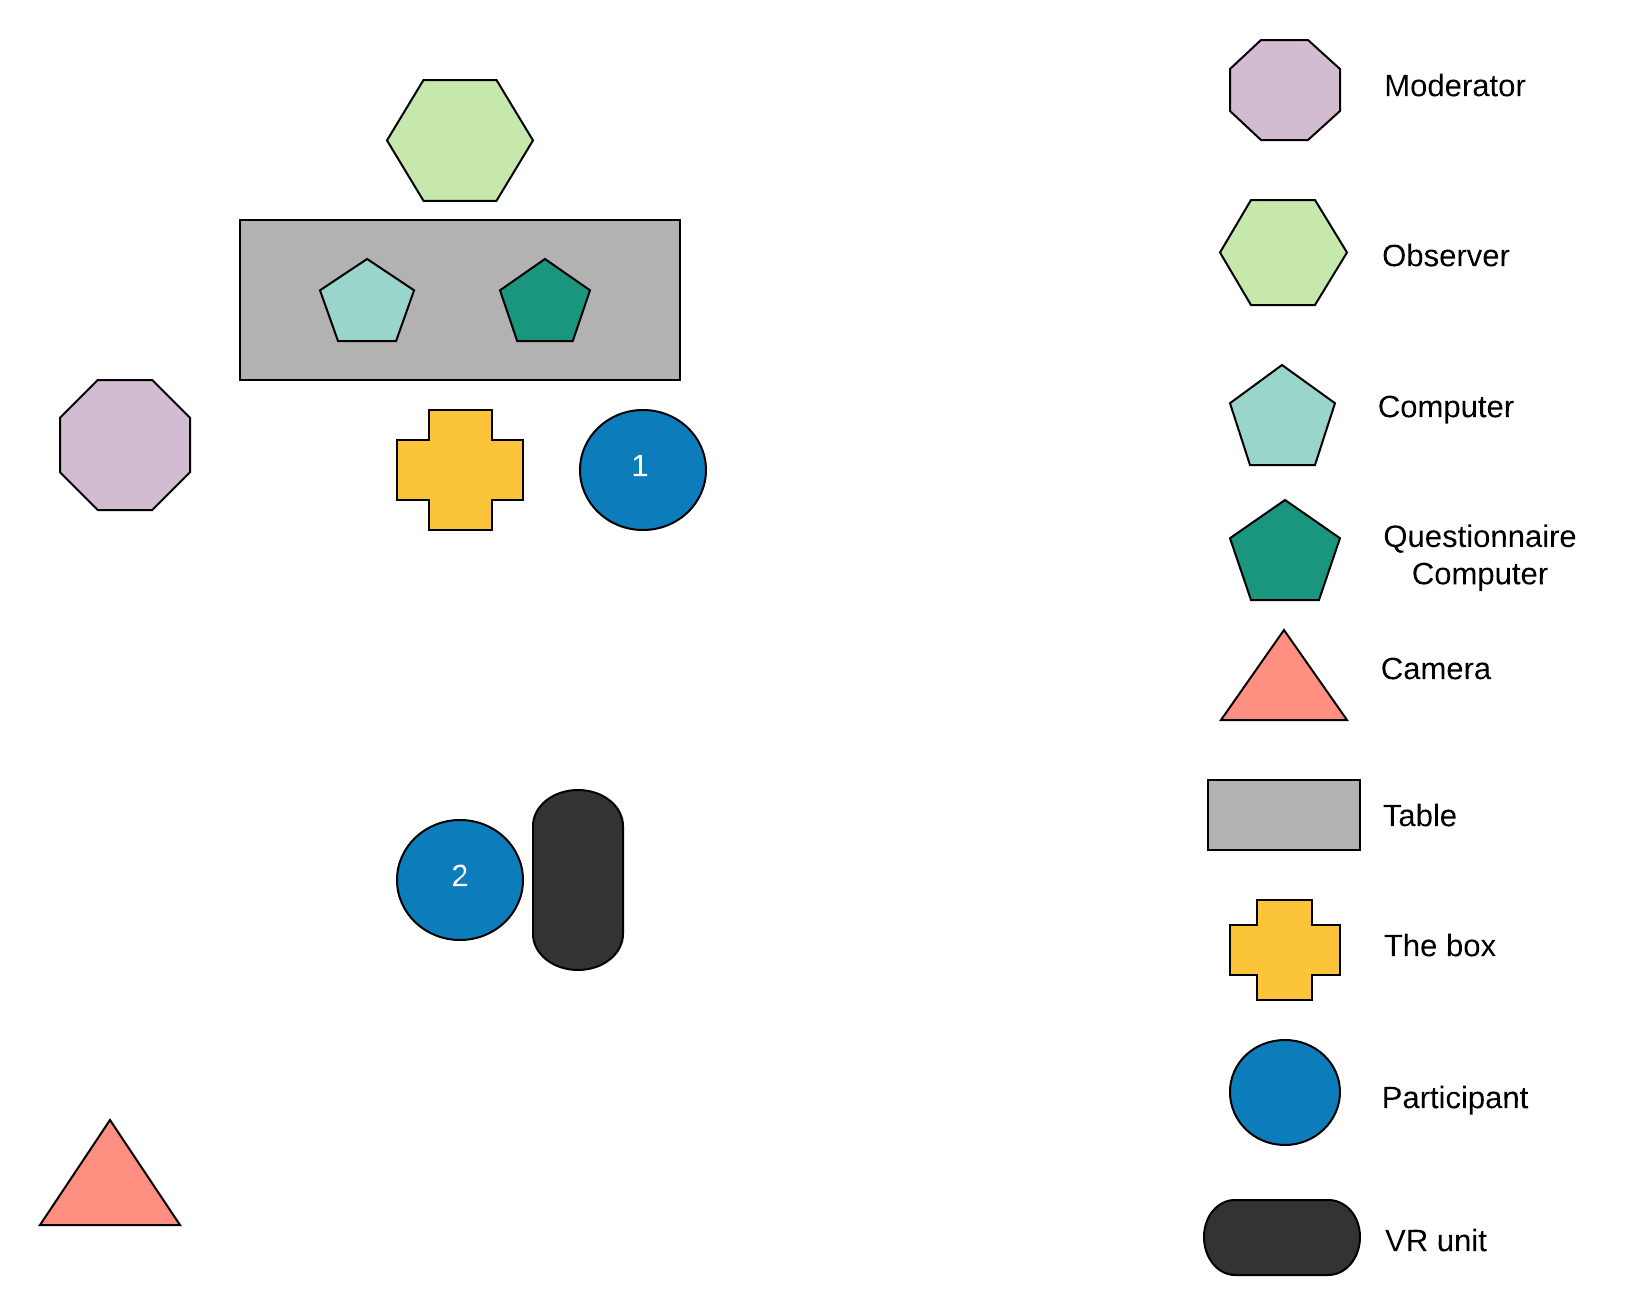
\includegraphics[width=1\linewidth]{figure/Evaluation/Test1.png}
	\caption{Our test setup, with the location of the participant, moderator, video camera and equipment. The two phases are visualized by the numbers in the circles.}
	\label{fig:test1}
\end{figure}

\subsection*{The equipment being used during the test}
\begin{itemize}
	\item[-] A camera running on a computer
	\item[-] The box where the tokens is placed with a camera inside
	\item[-] Laptop for filling out a questionnaire
	\item[-] HTC vive VR unit
\end{itemize}

\subsection*{Location and schedule}
The test took place Thursday 7/12 2017 in our group room at Aalborg University Copenhagen on Frederikskaj 12. Each testing with evaluation took approximately 15 to 20 minutes.

\subsection*{Test procedure}
Firstly, the participant was informed about the general purpose of the test, tasks and that they would give their consent to being filmed. After agreeing to this, the participant was asked to take the role of a client or an architect. Then they where asked to act like they needed a new garden and find out how the design should look. The client would take on the VR goggles and the architect would make a design with the markers with the help from the client. Afterwards the participants would switch roles and do the same thing again.

*Insert steps here*\\

After the participants tried their different roles they where asked to fill out a questionnaire (see appendix ??) as their respective roles, so each participant had to fill out two questionnaires. The questionnaires contained questions regarding the experience as a client and an architect.

\subsection{Results}
In this section we will display the results conducted from our questionnaires that the participants filled out after each role in the test (see \autoref{fig:boxPlotResults} and \autoref{fig:boxPlotResults2}). The questionnaires was not 100\% Likert scale questions, but we took those out and put them in a box plot. Some of the questions will be picked out and shown in a bar chart.
The questions is as follows:\\

Client Questions:\\
\begin{enumerate}
\item Rate the amount of discomfort you experienced during the test.
\item Was the framerate (the frequency at which the screen updates) tolerable?
\item How engaged did you feel with the program?
\item How good did the environment and objects look?
\item Did you feel you had enough space to move around?
\item Could you easily communicate with the other participant?
\end{enumerate}


\begin{figure}[H]
	\centering
\begin{tikzpicture}
\begin{axis}
[
boxplot/draw direction=y,
height=10cm,
width=15cm,
enlargelimits=0.03,
ytick={1,1.5,2,2.5,3,3.5,4,4.5,5},
xtick={1,2,3,4,5,6},
xlabel=Questions,
ylabel={Level of agreement},
xticklabels={
	1,2,3,4,5,6}
]
\addplot+[boxplot]
table[row sep=\\,y index=0] {
	data\\ 1\\ 1\\ 1\\ 2\\ 2\\ 2\\ 3\\ 4\\
};
\addplot+[boxplot]
table[row sep=\\,y index=0] {
	data\\ 2\\ 2\\ 2\\ 3\\ 4\\ 5\\ 5\\ 5\\
};   
\addplot+[boxplot]
table[row sep=\\,y index=0] {
	data\\ 4\\ 4\\ 4\\ 4\\ 4\\ 4\\ 4\\ 5\\ 
};   
\addplot+[boxplot]
table[row sep=\\,y index=0] {
	data\\ 2\\ 3\\ 4\\ 4\\ 4\\ 5\\ 5\\ 5\\
};  
\addplot+[boxplot]
table[row sep=\\,y index=0] {
	data\\ 2\\ 2\\ 3\\ 3\\ 3\\ 5\\ 5\\ 5\\
};  
\addplot+[boxplot]
table[row sep=\\,y index=0] {
	data\\ 1\\ 1\\ 4\\ 5\\ 5\\ 5\\ 5\\ 5\\
};  
 
\end{axis}
\end{tikzpicture}
\caption{Box plot graph showing the result of the client scale questions.}
\label{fig:boxPlotResults}
\end{figure}

\subsection*{Was the framerate (the frequency at which the screen updates) tolerable?}
As seen in \autoref{fig:barChartFrame}, 3 of the 8 participants didnt find the framerate very tolerable. 1 participant found it somewhat tolerable and 3 participants found it very tolerable.

\begin{figure}[H]
	\centering
	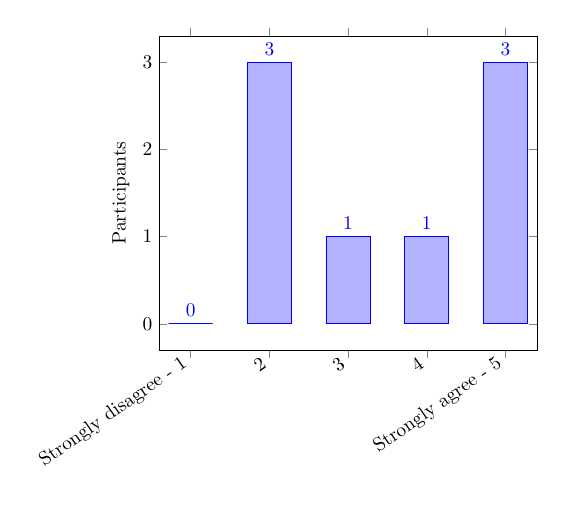
\begin{tikzpicture}[scale=0.7]
	\begin{axis}[ybar,bar width=0.8cm,enlargelimits=0.1,legend style={at={(0.5,-0.2)},anchor=north,legend columns=-1},ylabel={Participants},symbolic x coords={Strongly disagree - 1,2,3,4,Strongly agree - 5},xtick=data,nodes near coords,nodes near coords align={vertical},x tick label style={rotate=35,anchor=east},]
	\addplot coordinates {(Strongly disagree - 1,0) (2,3) (3,1) (4,1) (Strongly agree - 5,3)};
	\end{axis}
	
	\end{tikzpicture}
	\caption{Bar chart showing if the participants found the framerate tolerable.}
	\label{fig:barChartFrame}
\end{figure}


\subsection*{How engaged did you feel with the program?}
Out of 8 participants, 7 of them strongly agreed that they felt engaged with the program. This can be seen in \autoref{fig:barChartEngaged}

\begin{figure}[H]
	\centering
	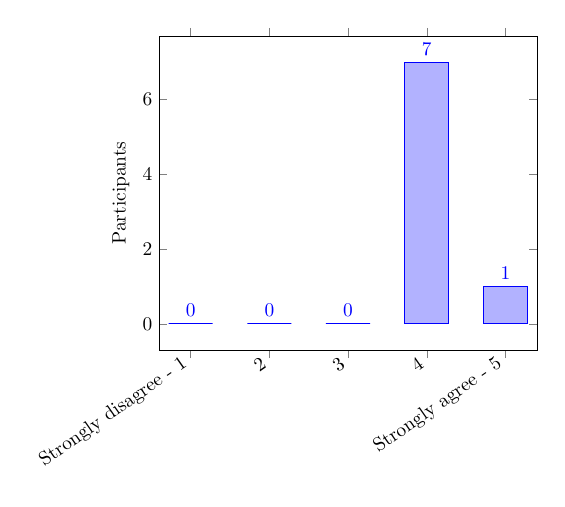
\begin{tikzpicture}[scale=0.7]
	\begin{axis}[ybar,bar width=0.8cm,enlargelimits=0.1,legend style={at={(0.5,-0.2)},anchor=north,legend columns=-1},ylabel={Participants},symbolic x coords={Strongly disagree - 1,2,3,4,Strongly agree - 5},xtick=data,nodes near coords,nodes near coords align={vertical},x tick label style={rotate=35,anchor=east},]
	\addplot coordinates {(Strongly disagree - 1,0) (2,0) (3,0) (4,7) (Strongly agree - 5,1)};
	\end{axis}
	
	\end{tikzpicture}
	\caption{Bar chart showing how engaged the participants felt like.}
	\label{fig:barChartEngaged}
\end{figure}


\subsection*{Could you easily communicate with the other participant?}
2 of the participants strongly disagreed that they were able to communicate with the other participant, where 6 of them strongly agreed that it was easy to communicate with the other participant. This can be seen in \autoref{fig:barChartCommunicate}.

\begin{figure}[H]
	\centering
	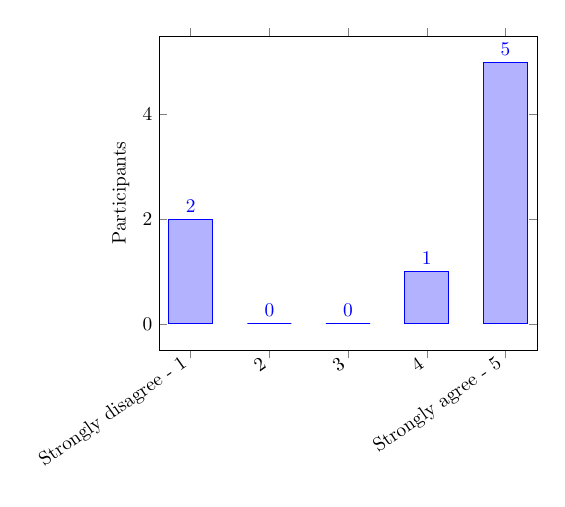
\begin{tikzpicture}[scale=0.7]
	\begin{axis}[ybar,bar width=0.8cm,enlargelimits=0.1,legend style={at={(0.5,-0.2)},anchor=north,legend columns=-1},ylabel={Participants},symbolic x coords={Strongly disagree - 1,2,3,4,Strongly agree - 5},xtick=data,nodes near coords,nodes near coords align={vertical},x tick label style={rotate=35,anchor=east},]
	\addplot coordinates {(Strongly disagree - 1,2) (2,0) (3,0) (4,1) (Strongly agree - 5,5)};
	\end{axis}
	
	\end{tikzpicture}
	\caption{Bar chart showing if it was easy to communicate with the other participant.}
	\label{fig:barChartCommunicate}
\end{figure}

Architect questions:\\
How easy was the product to use?\\
How easy was it to tell what the garden looked while you were building it?\\

\begin{figure}[H]
	\centering
\begin{tikzpicture}
\begin{axis}
[
boxplot/draw direction=y,
height=10cm,
width=15cm,
enlargelimits=0.03,
ytick={1,1.5,2,2.5,3,3.5,4,4.5,5},
xtick={1,2},
xlabel=Questions,
ylabel={Level of agreement},
xticklabels={
	1,2}
]
\addplot+[boxplot]
table[row sep=\\,y index=0] {
	data\\ 1\\ 3\\ 3\\ 4\\ 4\\ 5\\ 5\\ 5\\
};
\addplot+[boxplot]
table[row sep=\\,y index=0] {
	data\\ 1\\ 1\\ 2\\ 2\\ 2\\ 3\\ 3\\ 3\\
};   


\end{axis}
\end{tikzpicture}
\caption{Box plot graph showing the results of the architect Likert questions.}
\label{fig:boxPlotResults2}
\end{figure}


\subsection*{How easy was the product to use?}
Out of 8 participants 1 of them strongly disagreed that the product was easy to use, while 2 participants hit the middle ground and 5 participants agreed that the product was easy to use. This can be seen in \autoref{fig:barChartEasy}.

\begin{figure}[H]
	\centering
	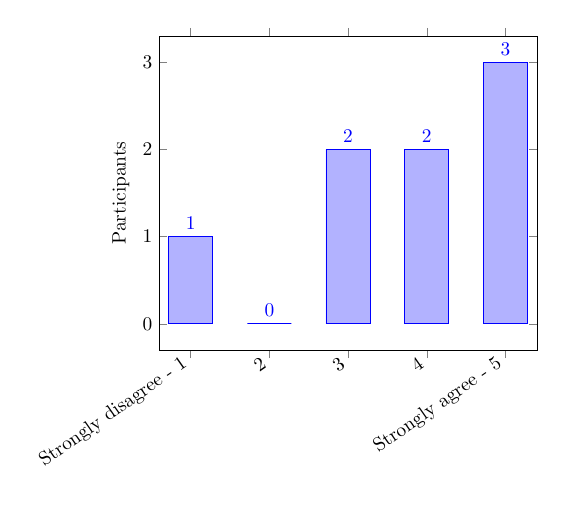
\begin{tikzpicture}[scale=0.7]
	\begin{axis}[ybar,bar width=0.8cm,enlargelimits=0.1,legend style={at={(0.5,-0.2)},anchor=north,legend columns=-1},ylabel={Participants},symbolic x coords={Strongly disagree - 1,2,3,4,Strongly agree - 5},xtick=data,nodes near coords,nodes near coords align={vertical},x tick label style={rotate=35,anchor=east},]
	\addplot coordinates {(Strongly disagree - 1,1) (2,0) (3,2) (4,2) (Strongly agree - 5,3)};
	\end{axis}
	
	\end{tikzpicture}
	\caption{Bar chart showing if the product was easy to use.}
	\label{fig:barChartEasy}
\end{figure}


\subsection*{How easy was it to tell what the garden looked liked while you were building it?}
5 participants disagreed that that it was easy to tell how the garden looked, while 3 participants hit the middle ground. This is seen in \autoref{fig:barChartLook}.

\begin{figure}[H]
	\centering
	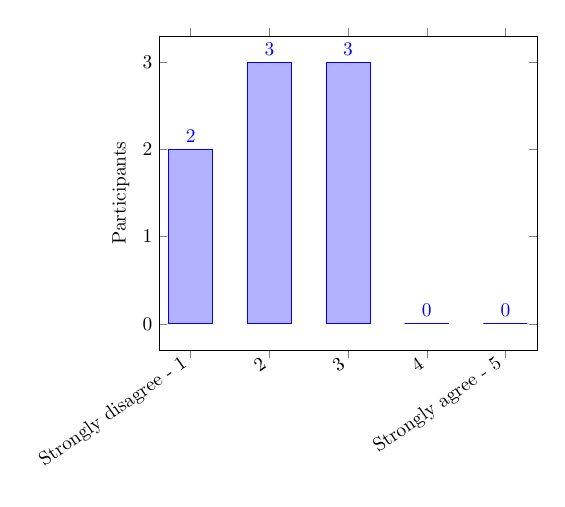
\begin{tikzpicture}[scale=0.7]
	\begin{axis}[ybar,bar width=0.8cm,enlargelimits=0.1,legend style={at={(0.5,-0.2)},anchor=north,legend columns=-1},ylabel={Participants},symbolic x coords={Strongly disagree - 1,2,3,4,Strongly agree - 5},xtick=data,nodes near coords,nodes near coords align={vertical},x tick label style={rotate=35,anchor=east},]
	\addplot coordinates {(Strongly disagree - 1,2) (2,3) (3,3) (4,0) (Strongly agree - 5,0)};
	\end{axis}
	
	\end{tikzpicture}
	\caption{Bar chart showing how easy it was to tell how the garden looked like, while building it.}
	\label{fig:barChartLook}
\end{figure}

Besides the Likert scale questions, we also asked some yes/no questions, where some of them will be illustrated in pie charts. 


\subsection*{Were you able to do everything you and the client wanted?}
As seen in \autoref{fig:pie1} over half of the participants answered yes to this question, and a little under half of them answered no.

\begin{figure}[H]
	\centering
	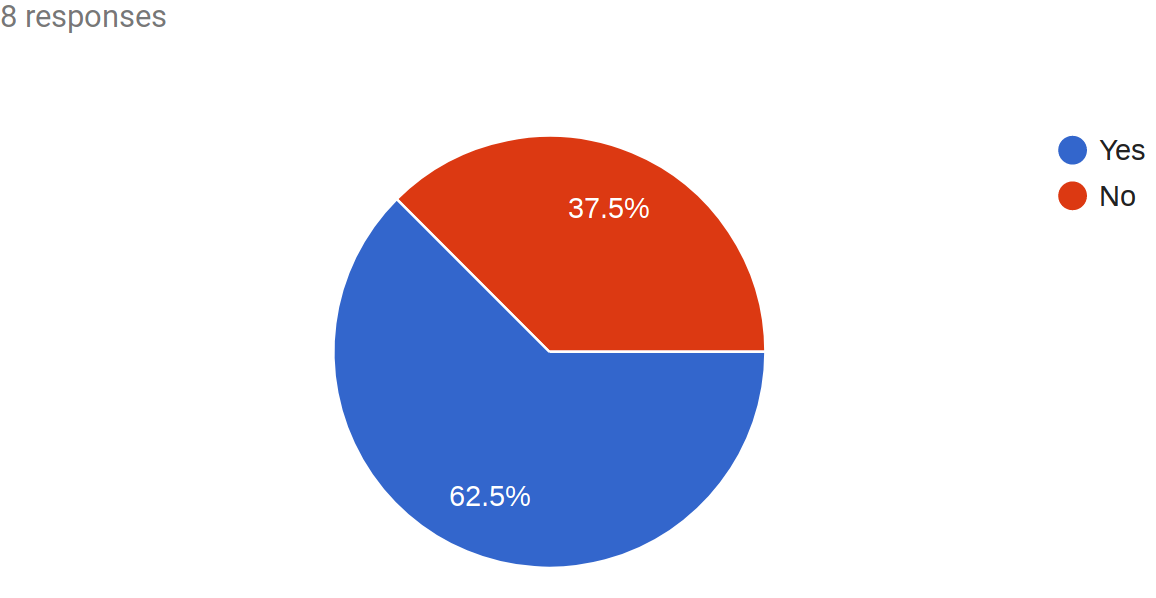
\includegraphics[width=0.9\linewidth]{figure/Evaluation/pie1.png}
	\caption{}
	\label{fig:pie1}
\end{figure}

In addition to this question the participants were able to give a comment, if they answered no to the given question. Here are some examples of the answers:\\

 \begin{quote}
 	
\textit{I had a hard time knowing where the client was on the glass plate compared to the items. Sometimes there were some consistency in where i placed the item and where it appeared, but i got the hang of it eventually}\\
  \end{quote}
  
  \begin{quote}
  \textit{Orientation is very difficult to understand}\\
  \end{quote}	
 	 
 	As it can be seen from the given answers, some of the participants had a hard time figuring out where the client was in the garden, which made it difficult for them to know where to place the objects in regards to the client.
 

\subsection*{Was it easy to follow the clients instructions?}
A little over half of the participants found it easy to follow the clients instructions, whereas a little under half of them did not find it easy. This can be seen in \autoref{fig:pie2}.

\begin{figure}[H]
	\centering
	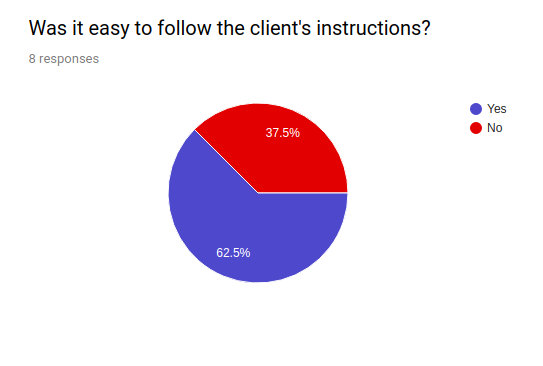
\includegraphics[width=0.9\linewidth]{figure/Evaluation/pie2.png}
	\caption{.}
	\label{fig:pie2}
\end{figure}

\subsection*{Did the program respond accurately to your actions?}
As it can be seen in \autoref{fig:pie3}, half of the participants stated that the program responded accurately to their actions and half of them stated that this was not the case.

\begin{figure}[H]
	\centering
	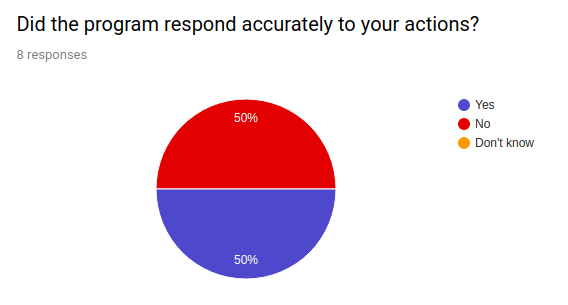
\includegraphics[width=0.9\linewidth]{figure/Evaluation/pie3.png}
	\caption{.}
	\label{fig:pie3}
\end{figure}

In addition to this question, we asked the participants who answered no to this question, to elaborate on their answer:\\

\begin{quote}
	\textit{It bugged out, so it did not show the items in VR}\\
\end{quote}

\begin{quote}
	\textit{No rotation}\\
\end{quote}

As seen above, one of the participants had some issues with the prototype bugging, and sometimes not showing the object in the VR world. Others complained that it was not possible to rotate the objects, which resulted in the client not having to see how the garden would look like exactly.


\subsection{Findings}
In general the participants were positive about our prototype, the Likert scale questions showed an overall understanding of our prototype.
Especially in \autoref{fig:barChartEngaged} it can be seen that all 8 participants felt engaged with the program, when they were in the VR environment. This could have something to do with the result of the question in \autoref{fig:barChartFrame}, a majority of the participants answered that the framerate was tolerable.\\


A fair amount of participants answered that they were able to do what the clients wanted as seen in \ref{fig:pie1}. A common statement from the participants were that it was difficult for them to localize the client in the garden. The architect couldn't see where the client was in the garden, because the client was able to move around freely inside the VR garden. Its hard to say how relevant this is, but it is still important to have in mind.\\


Over half of the participants answered that it was easy to follow the clients instructions (see \autoref{fig:pie2}) despite there being some problems with the prototypes functioning from time to time. Because we did not use a follow up question for this one we cant directly say why the last bit of the participants had difficulties following the clients instructions. Taking in consideration that the client and the architect stood almost right beside each other, it is most likely not a lack of communication, but rather a problem from the prototypes side.\\
Even though the above question was not elaborated further, the next given question, seen in \ref{fig:pie3} shows that half of the participants felt that the program responded to their actions, and half of them felt the opposite. This i very likely to have something to do with the prototype since some of the participants stated further that the prototype bugged out and didn't show the objects in VR. Another answer was that the objects didn't have any rotation, which made it hard to make the garden as detailed as possible or at least as finished as possible.



\section{Immersion test}
This immersion test was conducted to make a proof of our concept, to make sure that our idea of the prototype was plausible.

\subsection{Test goals}
The goal of the test was to determine if the prototype in fact did answer the final problem statement (\autoref{sec:FPS}). The keywords from the FPS are:
\begin{itemize}
	\item[-] Fast
	\item[-] Efficient
	\item[-] Immersive
\end{itemize}
and hence these were the words we were keen on measuring with this test.
\subsection{Sampling}
Finding real garden architects among the students at AAU CPH, turned out to be a larger challenge than first expected, and therefore it was decided that convenience sampling were to replace that criteria. Convenience sampling among the students at AAU CPH gave us a "random" assortment of test participants. In total, twelve participants were found.

\subsection{Test specifics}
The test consisted of three parts:
\begin{itemize}
	\item[-] 2D sketching
	\item[-] 3D viewing
	\item[-] Virtual reality
\end{itemize}
Between each part, the participant filled out the same questionnaire, changing their answers depending on what test they had just done. Each participant was given a test subject id, starting from 1, and going to 12. To eliminate bias we used every possible sequence combination of 2D sketching, 3D viewing and Virtual Reality on two differently designed gardens, as seen in \autoref{table:immersionCombinations}.

\begin{table}[H]
	\centering
	\caption{All the sequence combinations of 2D sketching, 3D viewing and virtual reality, and which participant that did what combination.}
	\label{table:immersionCombinations}
	\begin{tabular}{l | c|c|c|c|c|c}
		&
		\begin{tabular}[c]{@{}c@{}}VR\\ 2D\\ 3D\end{tabular} & \begin{tabular}[c]{@{}c@{}}VR\\ 3D\\ 2D\end{tabular} & \begin{tabular}[c]{@{}c@{}}2D\\ 3D\\ VR\end{tabular} & \begin{tabular}[c]{@{}c@{}}2D\\ VR\\ 3D\end{tabular} & \begin{tabular}[c]{@{}c@{}}3D\\ VR\\ 2D\end{tabular} & \begin{tabular}[c]{@{}c@{}}3D\\ 2D\\ VR\end{tabular} \\ \hline 
		Garden 1 & 2                                                                            & 5                                                                            & 4                                                                            & 3                                                                            & 1                                                                            & 6                                                                            \\ 
		Garden 2 & 7                                                                            & 8                                                                            & 9                                                                            & 10                                                                           & 11                                                                           & 12                                                                           \\
	\end{tabular}
	
\end{table}
The 2D sketches the participants were asked to study can be seen in \autoref{fig:sketchGarden1} and \autoref{fig:sketchGarden2}. These were both created from the 3D virtual scenes made in unity. The two gardens purposely have two very different layouts, and two very different complexity levels(The number of objects in the scene). This was done in another attempt to eliminate bias and the odds of the results being up to chance.
\begin{multicols}{2}
\begin{figure}[H]
	\centering
	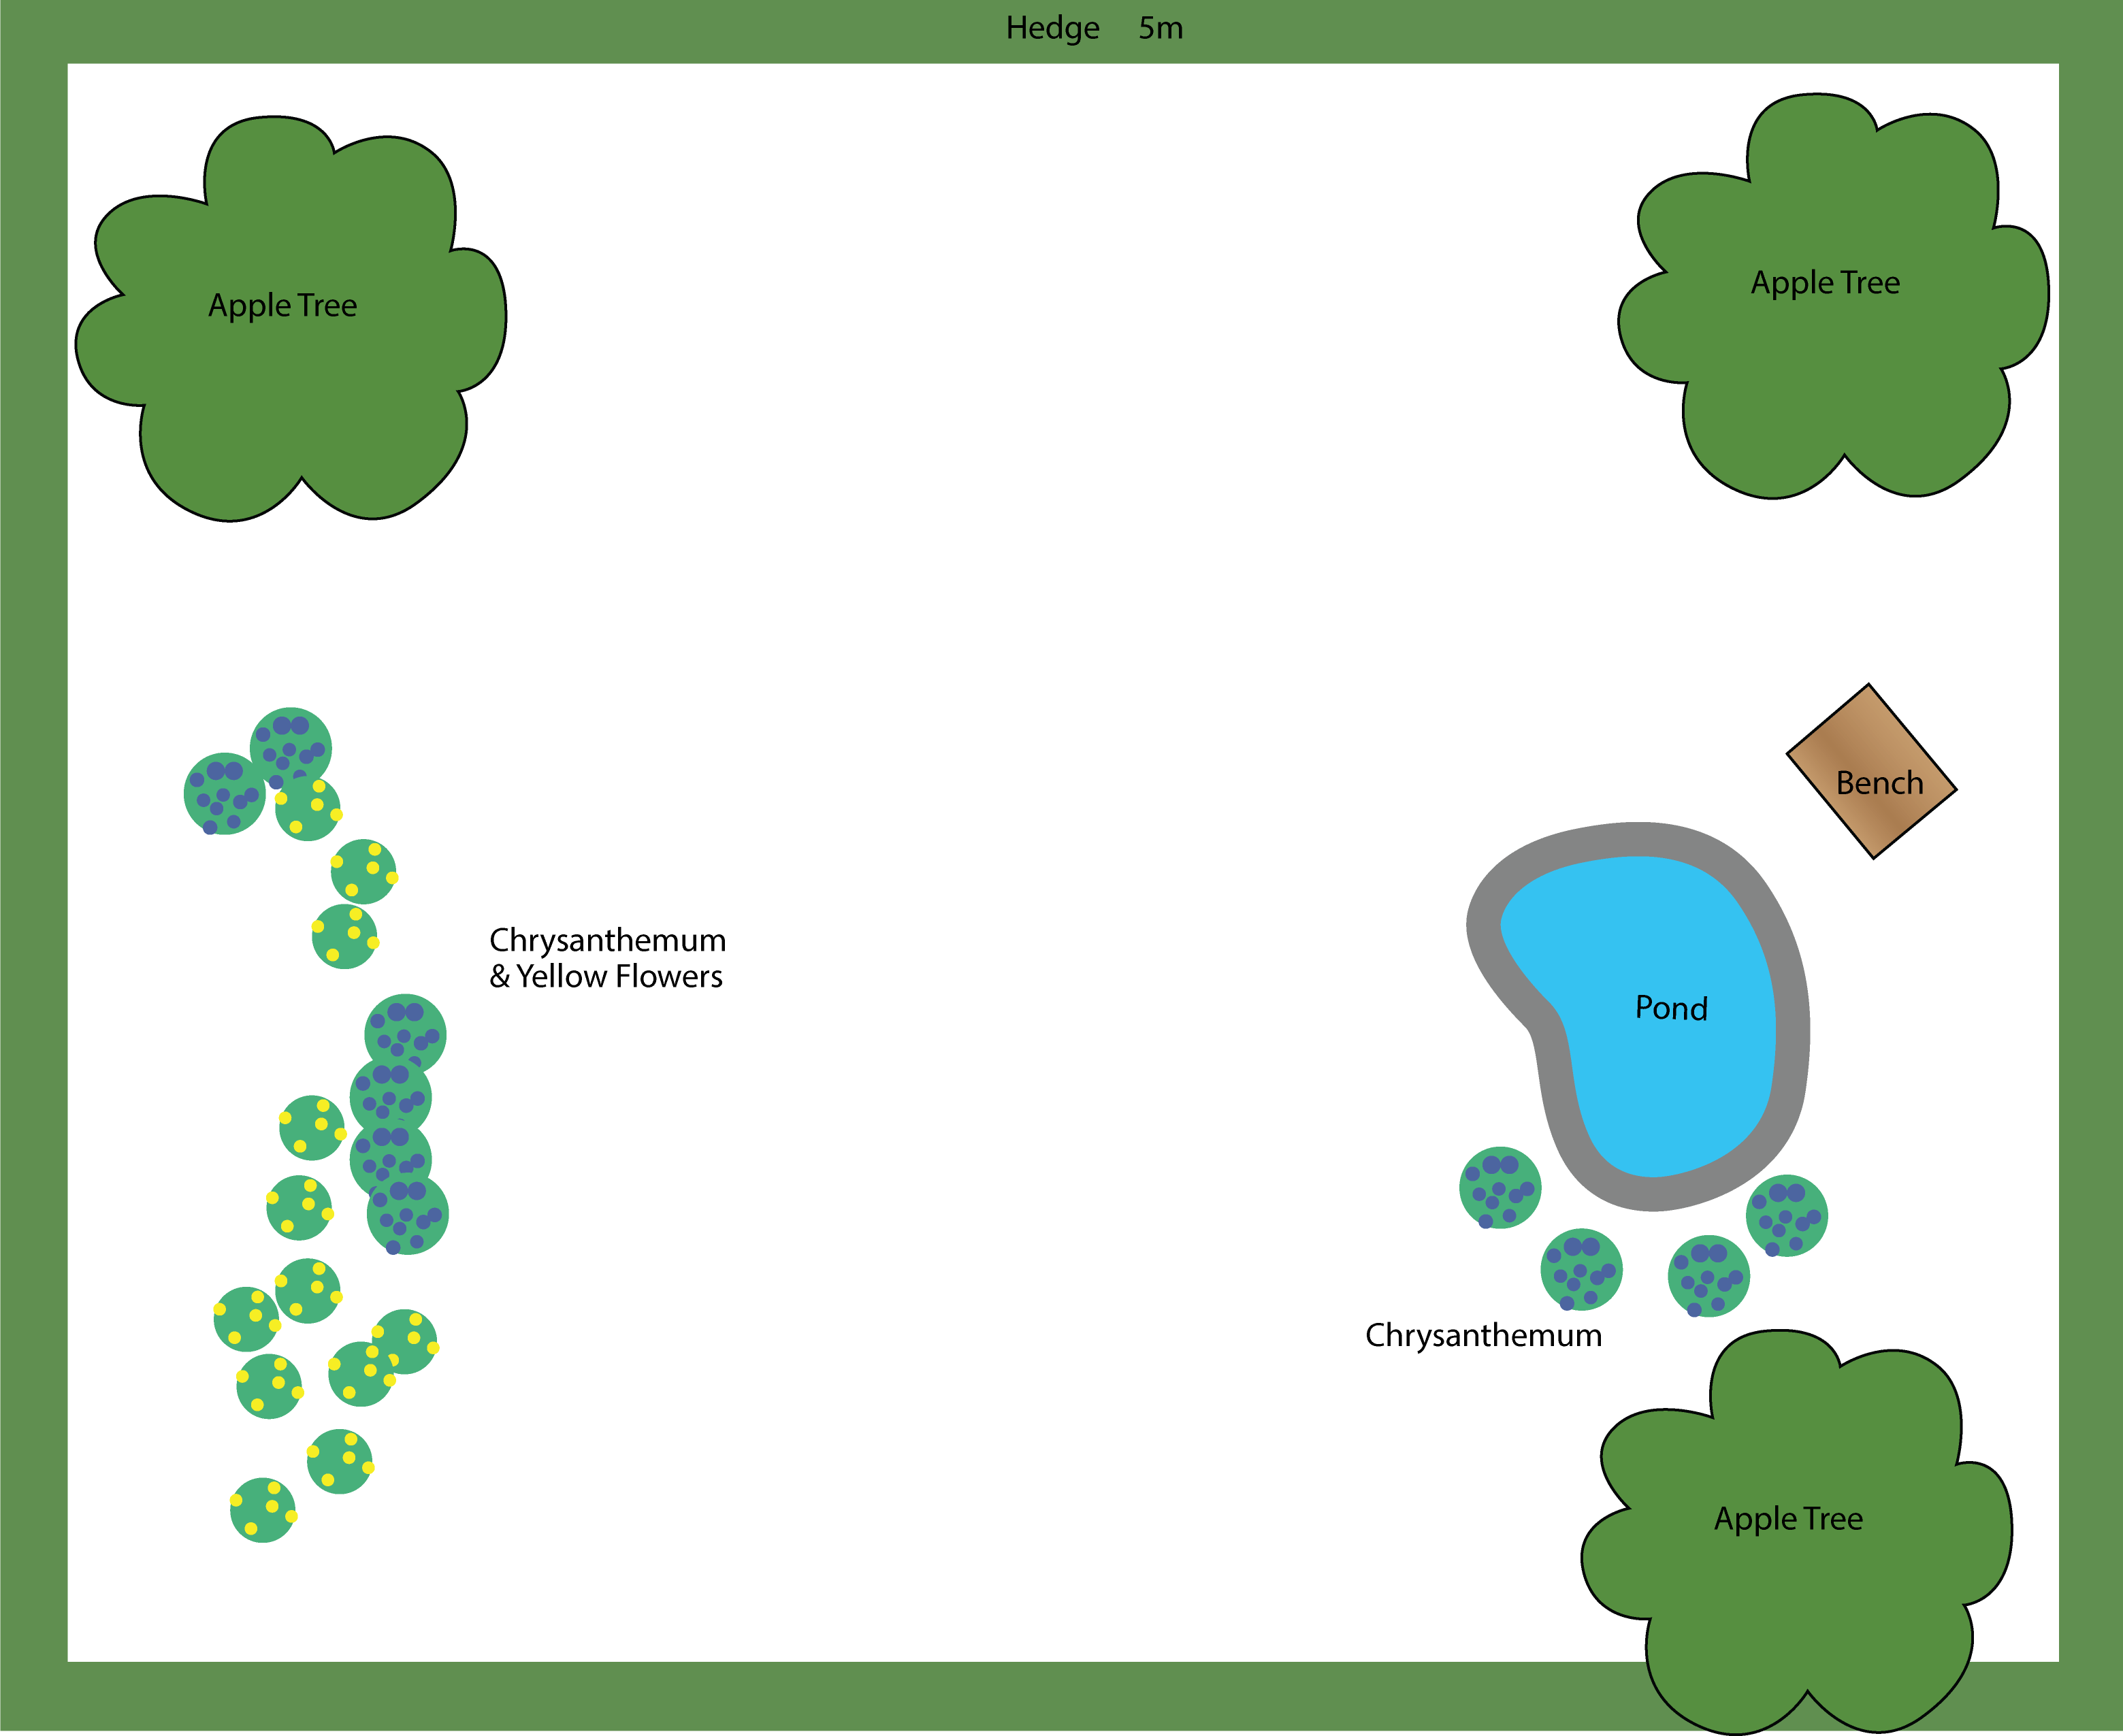
\includegraphics[width=1.0\linewidth]{figure/Evaluation/Garden1.png}
	\caption{Sketch garden 1}
	\label{fig:sketchGarden1}
\end{figure}
\columnbreak
\begin{figure}[H]
	\centering
	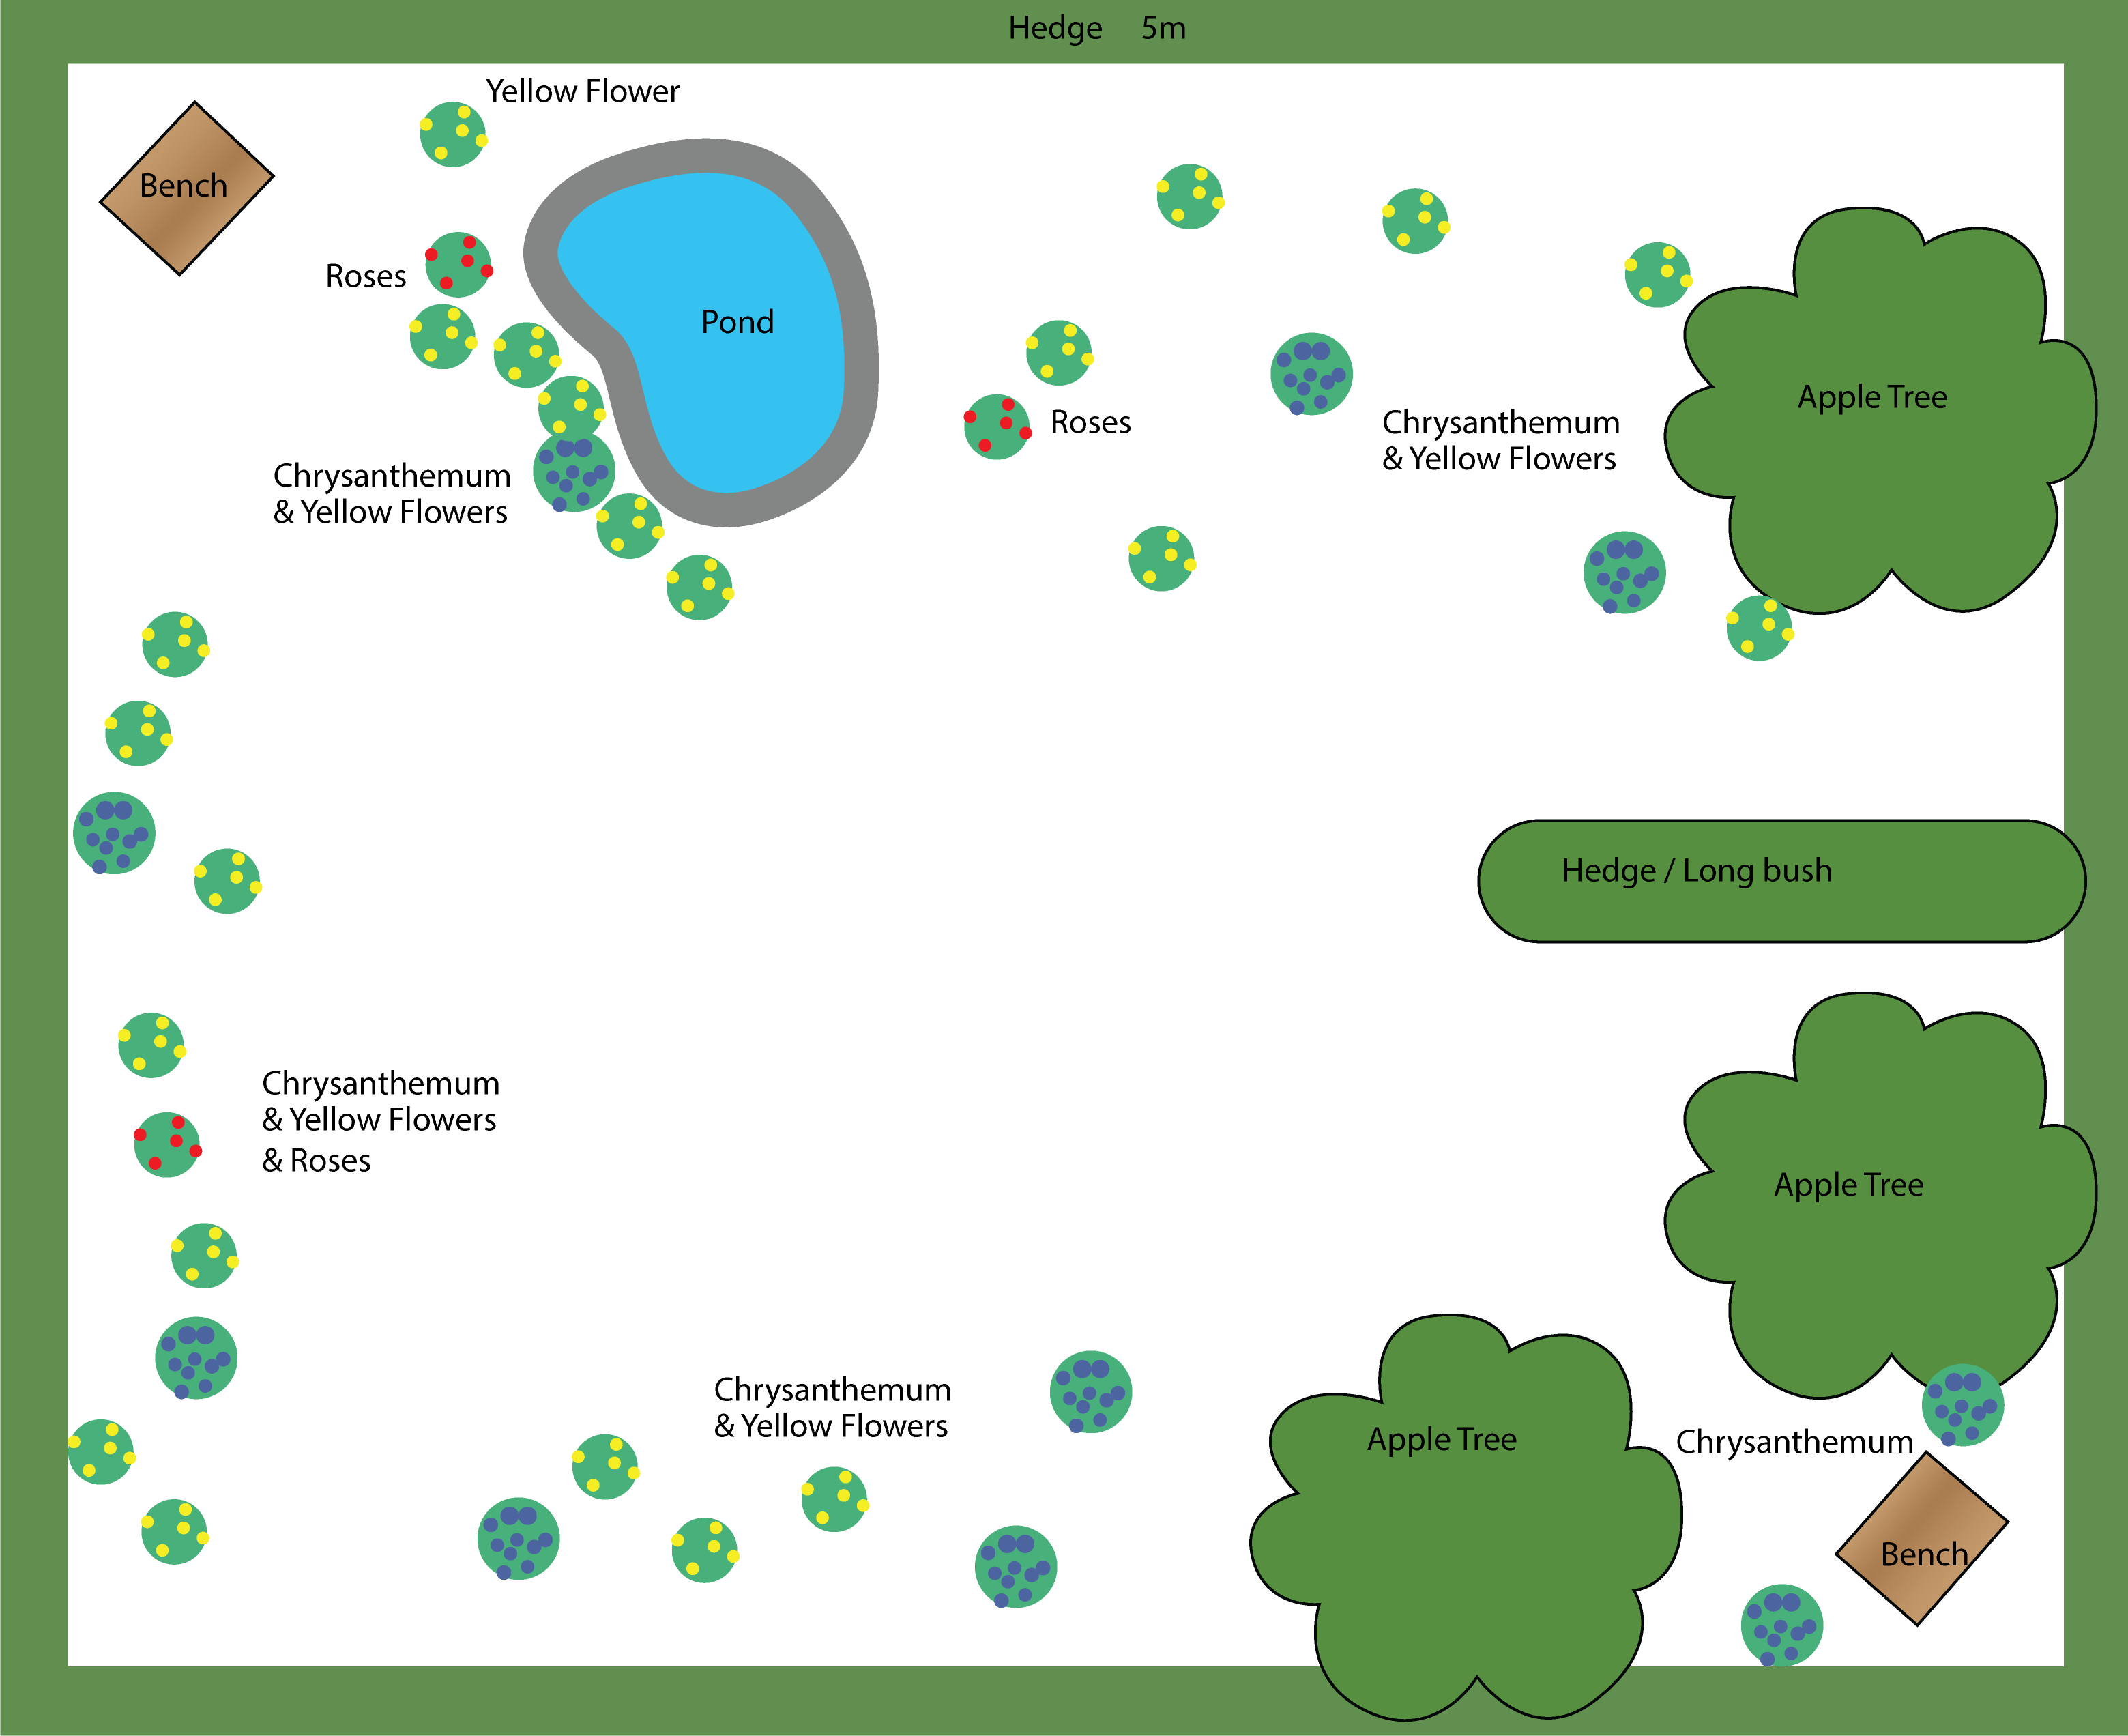
\includegraphics[width=1.0\linewidth]{figure/Evaluation/Garden2.png}
	\caption{Sketch garden 2}
	\label{fig:sketchGarden2}
\end{figure}
\end{multicols}
The 3D scenes had a camera that automatically moved and looked around the garden. This was done to replicate what we observed some garden architects were advertising on their web pages.

\subsection{Findings}
\begin{table}[H]
	\centering
	\caption{Average of responses}
	\label{table:averageResponse}
	\begin{tabular}{p{3cm}|p{3cm}|p{2cm}|p{3cm}|p{3cm}}
		Test type       & How long do you think it took you to gain insight into how it would be, to be in the garden? & How immersed did you feel? & How useful do you think this tool could be for a garden architect? & How much do you feel like you understood the garden's design? \\ \hline
		&&&&\\
		3D Viewing      & 6.08  & 4.67  & 4.00    & 8.67               \\
		Sketching       & 6.75    & 2.00    & 3.92      & 7.58            \\
		Virtual Reality & 8.17     & 7.67     & 4.58      & 9.17    
	\end{tabular}
\end{table}


All but 1 participant answered the final question prompting a comparison between the three different mediums. 
The contents of the comments have been separated into statements about the individual mediums:

8 out of 12 participants left a comment on what could be changed for 3D viewing. Of those, 7 comments concerned the ability to navigate or interact with the environment themselves. One comment said it would be beneficial to see the dimensions of the objects in the garden.x	

Of the sketching comments, 9 of 12 testers left a comment. Five comments said they wouldn't change anything or didn't know what they'd change. Two comments said they needed more depth to the image. One tester wanted a more detailed sketch, and one asked for a "more immersive experience" The tester who left the last comment started with the 2D sketch as the first medium for visualization and may have found the immersion question silly. 

As for the Virtual Reality test, 9 out of 12 testers left a comment. 1 of the 9 didn't know what could be improved. 1 person wanted elements like floor plans. Two wanted improved graphics. One person wanted a note taking functionality, the ability to highlight objects, and multi-user functionality. Two users wanted more interactivity, and two users wanted a larger area to walk around, as to remove the need for teleportation.

All but 1 participant answered the final question prompting a comparison between the three different mediums. 
The contents of the comments have been separated into statements about the individual mediums:
\begin{multicols}{2}
	\begin{table}[H]
		\centering
		\caption{3D Comments I guess}
		\label{my-label}
		\begin{tabular}{p{5cm}|c}
			Comment & Count \\ \hline
			Bad to not have control & 3 \\
			Some immersion & 3 \\
			Fast overview &2 \\
			Lacking some immersion &2 \\
			Felt polished& 1 \\
			Lack of dimensions& 1 \\
			Good for angles& 1 \\
			Lack of depth perception& 1 \\
			Movement confusing& 1 \\
			Strange& 1 \\
			Good idea of layout& 1 \\
		\end{tabular}
	\end{table}
	
	
\columnbreak

\begin{table}[H]
	\centering
	\caption{2D Comments I guess}
	\label{my-label}
	\begin{tabular}{p{5cm}|c}
		Comment & Count \\ \hline
		Quick & 3 \\
		Descriptive & 2\\
		Not immersive & 2 \\
		Good for accurate positions & 2 \\
		Good overview  & 2 \\
		Easy to understand & 2 \\
		Difficult to visualize & 1 \\
		Inaccurate& 1 \\
		Good for sizes & 1 \\
	\end{tabular}
\end{table}
\end{multicols}



\begin{table}[H]
	\centering
	\caption{VR Comments I guess}
	\label{my-label}
	\begin{tabular}{p{5cm}|c}
		Comment & Count \\ \hline
		Good for immmersion & 7 \\
		Good feel of garden & 4 \\
		Good for size  & 2 \\
		Useful & 2 \\
		Lacking interactivity & 2 \\
		Good for angles & 1 \\
		Good for distances& 1 \\
		Lack of dimensions& 1 \\
		Good for focus on detail& 1 \\
		Limited FOV& 1 \\
		Natural& 1 \\
		Interesting& 1 \\
		Quick insight& 1 \\
		Low FPS& 1 \\
		Lack of overview& 1 \\
		Good for layout& 1 \\
		
	\end{tabular}

\end{table}

